In this section, we evaluate our algorithms on two datasets, a set of synthetic graphs and a set of graphs modeling active ingredients in antiviral drugs for the 
treatment of AIDS. We call the former the synthetic graph dataset and the later the real graph dataset. We perform two sets of tests; In the first set, we evaluate 
our algorithms on the retrieval of induced subgraph to query and In the second set, we evaluate retrieval of non induced sugraph to query.  To test the efficacy 
of our algorithm with regard to induced subgraph query, we evaluate the proposed algorithm in comparison with Messmer's Network Algorithm and a sequential SCAN 
using the state-of-the-art subgraph isomorphism detection algorithm VF2\cite{cordella2001_vf2}.
We also evaluate our algorithm with regard to non-induced subgraph query, where we compare proposed algorithm with the sequential scan only.
All the algorithms were implemented using the C++ programming language and run on a Intel Core i-3 CPU 3.09 GHZ, 16 Gbyte memory, Personal Computer running 
Windows 7 Professional Operating system.

\subsection{Graph Datasets}
We evaluate our algorithms by processing the retrieval of descriptors from the compounds dataset.
We use AIDS Antiviral Screen dataset to provide a real graph dataset.
This dataset contains around 43,000 chemical compounds and is available publicly from NCI
\footnote{National Cancer Institute http://dtp.nci.nih.gov/}.
We denote this dataset as ``AIDS'' in our experiment.
The graphs of AIDS have an average number of 25 vertices and 27 edges, a maximum of 438 vertices and 441 edges,
63 distinct vertex labels and 3 distinct edge labels.

In order to evaluate our algorithms over a larger database to test scalability, we use synthetic large dataset. The graph generator is configured to emit only connected graphs thathave an edge probability of 50 percent. Except where explicitly stated, 10 distinct vertex labels and 10 distinct.

\begin{figure}[h]
\centering
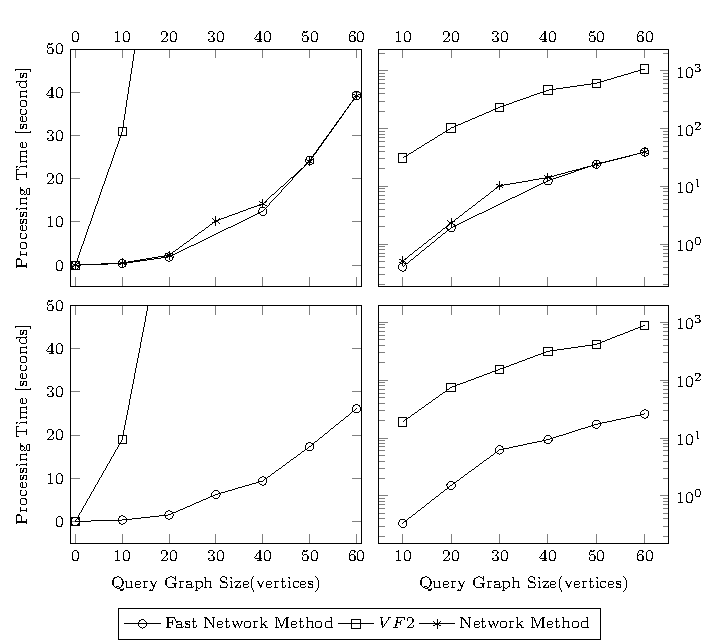
\includegraphics[width=1.0\textwidth]{images/realdataplot.pdf}
\caption{Real Data}
\label{fig:fig61}
\end{figure}
%\begin{figure}[t]
%\centering
%\epsfig{file=images/Ind_AID_Siz_Pro.eps, height=2in, width=3in}
%\caption{Processing Time for Induced Subgraph Isomorphism Query}
%\label{fig:fig3}
%\end{figure}
%\begin{figure}[t]
%\centering
%\epsfig{file=images/Typ_AID_Siz_Pro.eps, height=2in, width=3in}
%\caption{Processing Time for Subgraph Isomorphism Query}
%\label{fig:fig4}
%\end{figure}

\subsection{Chemical Descriptor Search}
In chemistry, substructures of compounds that imply a chemical, physical property of the compound are called as descriptor.
Fast retrievals of descriptors from compounds aids research of compounds.
We evaluate our algorihm by processing the retrievals of descriptors.
We builded a model graph database $D$ by extracting graph database $W$ composed of 10,000 compounds whose size are less than 40 from AIDS and applying frequent graph mining to $W$.
We set minimum support as 5 persents.
$D$ is composed of 18930 distictive frequent subgraphs.

We vary average size of query graphs and evaluate query processing time.
For each plot, 100 query graphs are extracted from $W$.
Query processing time is time to process the all query graphs and the time to construct the DAG is excluded.

Fig.\ref{fig:fig3} shows the processing time for induced subgraph isomorphism query.
Fig.\ref{fig:fig3} indicates that proposed algorithm has no improvements from Messmer et al.'s algorithm.
It is because that their are originally few decompositions that creates disconnected graphs and also few redundant subgraph isomorphism detections in DAG.
So in this experiment, our improvements did not work.

Fig.\ref{fig:fig4} shows the processing time for subgraph isomorphism query.
Fig.\ref{fig:fig4} indicates the subgraph isomorphism query is faster than SCAN same as Messmer et al's algorithm.

\subsection{Synthetic Data Search}
In chemical descriptor search, we can not show improvements of proposed algorithm in term of processing time.
In order to demonstrate improvements of proposed algorithm, we process subgraph isomorphism query on synthetic data.

We vary average size of query graphs and evaluate query processing time.
Model graph dataset is composed of 20,000 graphs whose average number of size are 10.
100 query graphs are generated for each plot.

\begin{figure}[h]
\centering
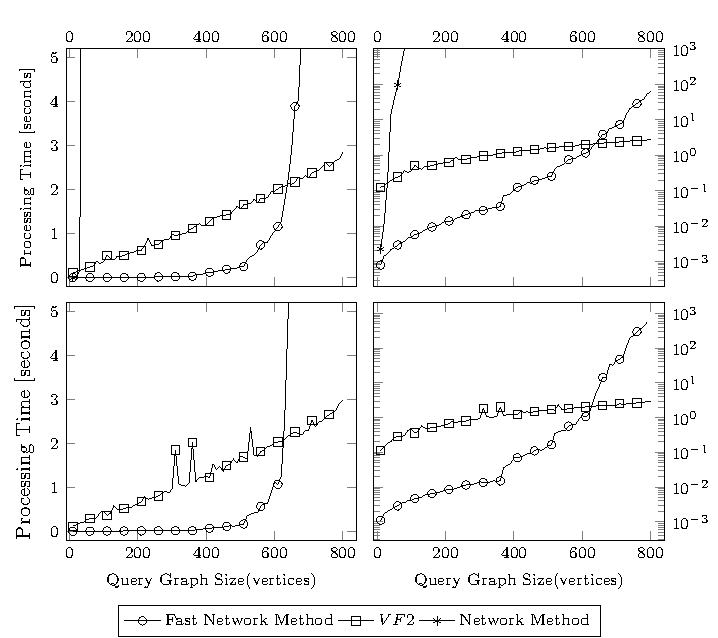
\includegraphics[width=1.0\textwidth]{images/syndataplot.pdf}
\caption{Synthetic Data}
\label{fig:fig61}
\end{figure}
%

Fig.\ref{fig:fig5} shows the processing time for induced subgraph isomorphism query.
Fig.\ref{fig:fig5} indicates that proposed algorithm is faster than Messmer et al.'s algorithm.
The processing time of proposed algorithm is stable against the variation of the size of query graphs.
On the contrary, the processing time of Messmer et al.'s algorithms is skyrockets when the size of query graphs becomes large.

%\begin{figure}[h]
%\centering
%\epsfig{file=images/Typ_Syn_Siz_Pro.eps, height=2in, width=3in}
%\caption{Processing Time for typical Subgraph Isomorphism Query}
%\label{fig:fig6}
%\end{figure}

%
\begin{figure}[h]
\centering
\centerline{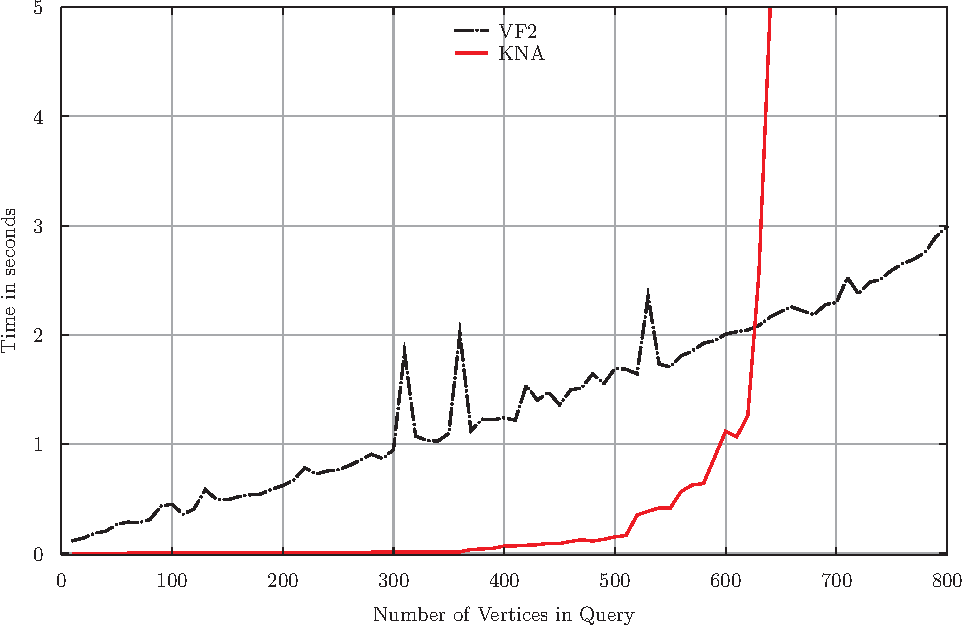
\includegraphics{images/kna_non_inducedS}}
\caption{Processing Time for Subgraph Isomorphism Query for Synthetic Data}
\label{fig:fig9}
\end{figure}

\begin{figure}[h]
\centering
\centerline{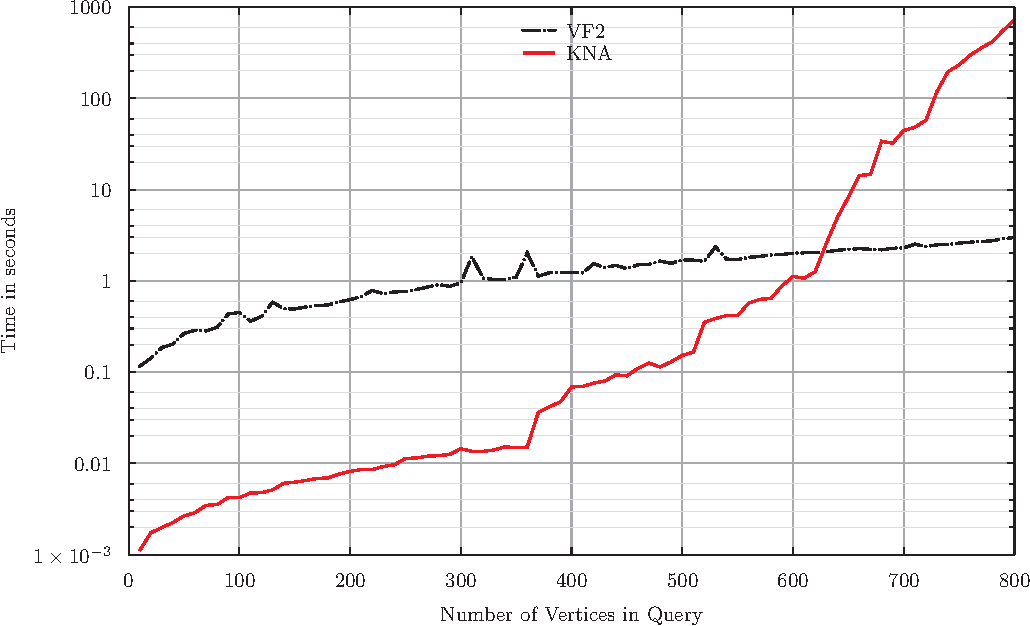
\includegraphics{images/kna_non_induced_logS}}
\caption{Logarithmic Plot of Processing Time for Subgraph Isomorphism Query for Synthetic Data}
\label{fig:fig10}
\end{figure}

\begin{figure}[h]
\centering
\centerline{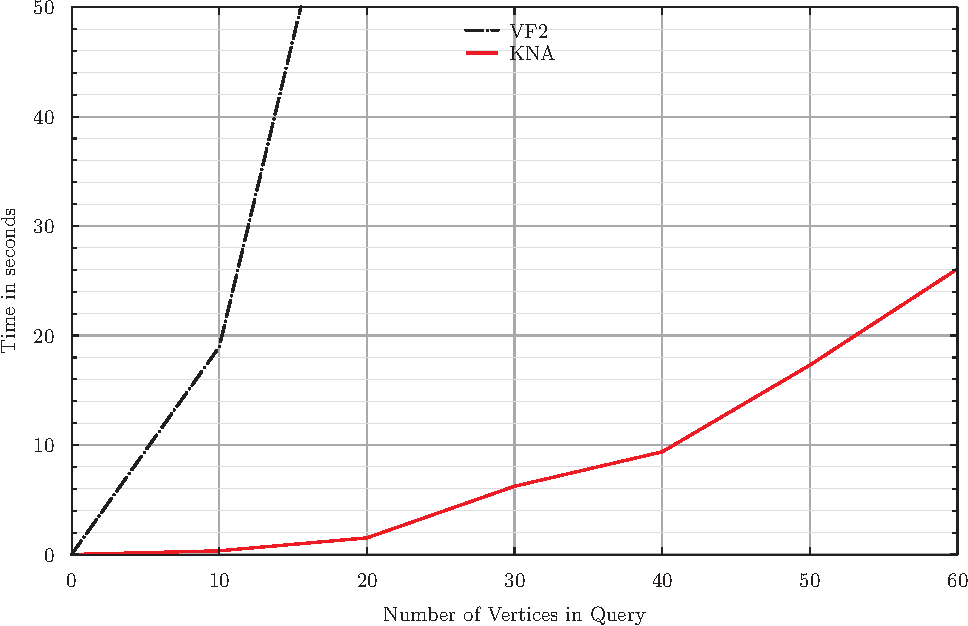
\includegraphics{images/kna_non_inducedR}}
\caption{Linear Plot of Processing Time for Subgraph Isomorphism Query for Real Data}
\label{fig:fig11}
\end{figure}

\begin{figure}[h]
\centering
\centerline{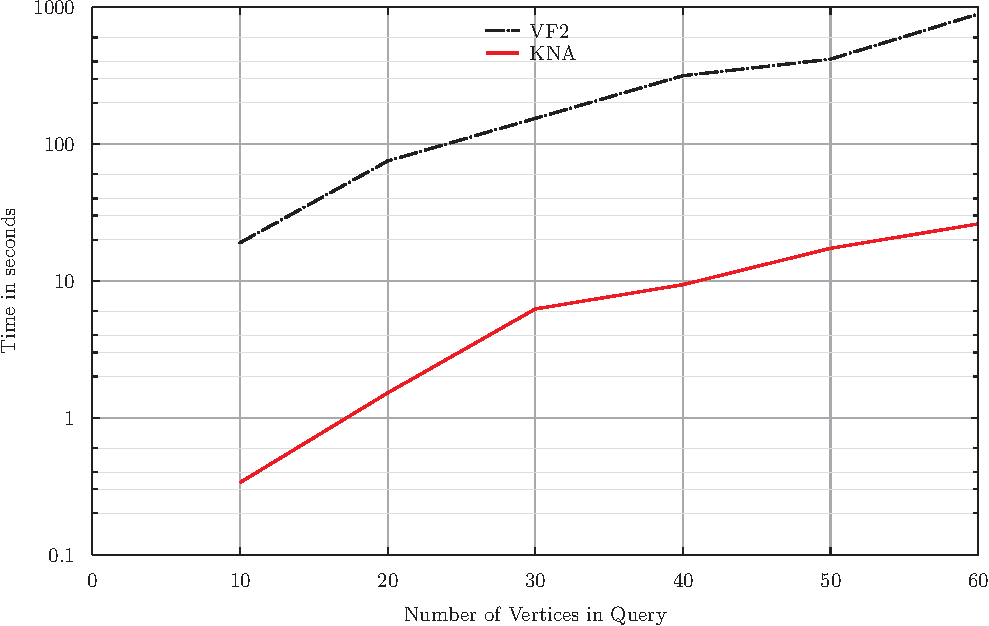
\includegraphics{images/kna_non_induced_logR}}
\caption{Logarithmic Plot of Processing Time for Subgraph Isomorphism Query for Real Data}
\label{fig:fig12}
\end{figure}


Fig.\ref{fig:fig6} shows the processing time for subgraph isomorphism query.
Fig.\ref{fig:fig6} indicates the subgraph isomorphism query is faster than SCAN same as Fig.\ref{fig:fig5}.

%\begin{figure}[h]
%\centering
%\epsfig{file=images/Ind_Syn_DAG_Con.eps, height=2in, width=3in}
%\caption{DAG Construction Time for Induced Subgraph Isomorphism Query}
%\label{fig:fig7}
%\end{figure}

We vary size of model graph database and evaluate the construction time of DAG.
Fig.\ref{fig:fig7} shows the construction time of DAG for induced subgraph isomorphism query.
The construction Time of DAG of proposed algorithm is almost same as the one of Messmer et al.'s algorithm.

%% \Subsection{Appendix}


%% \begin{algorithm}
%% \caption{New Network Algorithm, NNA($D , q$)}
%% \label{alg:alg05}
%% \begin{algorithmic}
%% \STATE Input: Model graphs in DAG, $D(G)= \{$($g_1 ,s_1 ,P_1 ,\{c^{'}_1 ,c^{''}_1 \},E$)$,\ldots,$($g_n,s_n,P_n,\{c_n^{'},c_n^{''}\},E_n$)$ \}$, Query $q$
%% \STATE and the set of all subgraphs in DAG, $G_{all} = \cup_{i=1}^n \{g_1 ,c_1^{'},c_1^{''},g_2 ,c_2^{'},c_2^{''}\ldots \}$ 
%% \STATE Output: $Z$, the set of all subgraph isomorphisms in Model graphs in $D$ to query $q$ 
%% \end{algorithmic}
%% \begin{algorithmic}[1]
%% \STATE $F \leftarrow \emptyset$
%% \STATE $Z \leftarrow \emptyset$
%% %%\FOR{ each $(g,s,P,\{c^{'},c^{''}\}) \in  D$}
%% \FOR{ each subgraph in $G_{all}$}
%%   \STATE  $s \leftarrow unsolved$
%% \ENDFOR
%% \FOR{ each $(g,s,P,\{c^{'},c^{''}\}) \in D$}
%%    \STATE $F \leftarrow $SubgraphQuery($g,s,P,\{c^{'},c^{''}\},q$)
%%    \IF{$F\neq \emptyset$}
%%       \STATE $Z \leftarrow Z \cup \{F\}$
%%    \ENDIF
%% \ENDFOR
%% \RETURN $Z$
%% \end{algorithmic}
%% \end{algorithm}


% LocalWords:  kna
